% ECE501 Digital Image Processing -- Week 8 Project Progress Report (Group 15)
% Build: tectonic main.tex
\documentclass[11pt,a4paper]{article}

\usepackage[margin=2.2cm]{geometry}
\usepackage[T1]{fontenc}
\usepackage{lmodern}
\usepackage{microtype}
\usepackage{amsmath,amssymb}
\usepackage{graphicx}
\usepackage{booktabs}
\usepackage{tabularx}
\usepackage{longtable}
\usepackage{array}
\usepackage{multirow}
\usepackage[table]{xcolor}
\usepackage{enumitem}
\usepackage{caption}
\usepackage{fancyhdr}
\usepackage{listings}
\usepackage{tikz}
\usepackage{placeins}
\usetikzlibrary{positioning,arrows.meta,fit,backgrounds}
\usepackage[colorlinks=true,linkcolor=blue!50!black,citecolor=blue!60!black,urlcolor=blue!60!black]{hyperref}

\definecolor{hdr}{HTML}{DCE6F2}
\definecolor{codebg}{HTML}{F6F8FA}
\definecolor{okgreen}{HTML}{1E7B34}
\definecolor{badred}{HTML}{B3261E}

\newcommand{\code}[1]{\texttt{\detokenize{#1}}}
\newcolumntype{L}{>{\raggedright\arraybackslash}X}
\newcolumntype{C}{>{\centering\arraybackslash}X}
\newcolumntype{R}{>{\raggedleft\arraybackslash}X}

\lstset{
  basicstyle=\ttfamily\footnotesize,
  backgroundcolor=\color{codebg},
  frame=single, rulecolor=\color{black!15},
  breaklines=true, columns=fullflexible,
  keywordstyle=\color{blue!60!black}\bfseries,
  commentstyle=\color{black!55}\itshape,
  stringstyle=\color{okgreen},
  showstringspaces=false,
  xleftmargin=2pt, xrightmargin=2pt
}

\captionsetup{font=small,labelfont=bf}
\setlist{itemsep=2pt,topsep=4pt}
\emergencystretch=3em

\pagestyle{fancy}
\fancyhf{}
\fancyfoot[C]{\small Group 15 \textbar\ Week 8 Project Progress Report \textbar\ Page \thepage}
\renewcommand{\headrulewidth}{0pt}

\begin{document}


\begin{center}
{\LARGE\bfseries Week 8 Project Progress Report}\\[4pt]
{\large\bfseries Adaptive Fabric Surface Defect Detection and Localization using\\ Classical Texture Descriptors}
\end{center}

\noindent
\textbf{Course Name:} ECE501 Digital Image Processing (DIP)\\
\textbf{Group Number:} Group 15\\
\textbf{Group Members:} Rinal Shah, Varun Hotani, Aadi Mehta, Pratik Agrawal\\
\textbf{Week Number:} Week 8\\
\textbf{Date:} November 12, 2026\\
\textbf{Deliverable:} Supervised classical detector at $16\times16$ windows and pixel level; strip-grouped cross-validated evaluation; final results\\
\textbf{Branch:} \code{feat/week-8}

\section*{Objectives of the Week}
\begin{itemize}
  \item Raise precision, recall, F1-score and IoU as far as the classical approach allows, evaluated without any leakage between training and test strips.
  \item Localize at $16\times16$ windows and at single pixels instead of $256\times256$ patches, so that 2--6\,px threads can be delineated.
  \item Close the project's method work and freeze the final configuration for the End-Semester report.
\end{itemize}

\section*{Summary of the Week}
\begin{center}
\renewcommand{\arraystretch}{1.15}
\begin{tabularx}{\textwidth}{@{}lL@{}}
\toprule
\textbf{Item} & \textbf{Outcome (real AFID, strip-grouped 5-fold CV, thresholds from validation strips only)} \\
\midrule
Pixel level & Pooled precision \textbf{52.3\,\%}, recall 25.8\,\%, F1 34.5\,\%, IoU \textbf{20.9\,\%} (Week~7 one-class: IoU 1.1\,\%). One weft-crack strip holds 48\,\% of all AFID defect pixels; without it, precision 52.2\,\%, recall 49.1\,\%, F1 \textbf{50.6\,\%}, IoU \textbf{33.9\,\%} \\
$16\times16$ windows & AUROC \textbf{0.980}; pooled precision 58.0\,\%, recall 35.0\,\%, F1 43.7\,\% \\
$256\times256$ patches & Pooled F1 \textbf{62.3\,\%} (Week~7: 23.0\,\%), patch AUROC 0.968 (Week~7: 0.536) \\
Image level & Accuracy \textbf{80.8\,\%} over 245 strips (75/105 defective found, 17/140 false alarms), F1 76.1\,\%, AUROC 0.865; \textbf{88.2\,\%} accuracy on fabric 03 \\
Method & GLCM + LBP + Gabor windows at $16\times16$ with multi-scale context and strip normalisation; per-pixel filter bank; Hough line linking; gradient-boosted trees; every choice made on validation strips \\
Quality & 103 tests; full results in \code{Results/final_supervised/} and \code{Results/AFID_results.xlsx} \\
\bottomrule
\end{tabularx}
\end{center}

%=====================================================================
\section*{Work Completed This Week}

\subsection*{A. Why a Supervised Detector}

Weeks~3--7 used \emph{one-class} models: a texture reference was fitted on defect-free strips, and anything far from it was flagged. Week~7's threshold-free diagnosis showed the limit of that idea. Within a defective strip, the reference ranked defect windows above normal ones only slightly better than chance (window AUROC 0.536), because the AFID capture shift moves the \emph{whole} strip away from the defect-free reference. AFID, however, ships a pixel mask for every defective strip. A classifier trained on those masks learns what \emph{defects} look like, not only what normal fabric looks like. The approach stays classical throughout:
\begin{itemize}
  \item the inputs are the same hand-crafted descriptors (GLCM \cite{haralick1973}, LBP \cite{ojala2002}, Gabor \cite{jain1991}) plus a classical per-pixel filter bank
  \item the decision function is gradient-boosted decision trees \cite{friedman2001,ke2017}
  \item nothing is learned end-to-end from raw pixels
\end{itemize}

\subsection*{B. Window Stage: $16\times16$ Windows with Multi-Scale Context}

Every $16\times16$ window (stride 8; about 11{,}300 per strip, 2.8 million over AFID) is described by a feature row:
\begin{equation}
\mathbf{x}_w=\Big[\underbrace{\mathbf{d}_{16}(w)}_{\text{GLCM+LBP+Gabor, 82-D}},\;
\underbrace{\mathbf{z}_{16}(w)}_{\text{same, strip-normalised}},\;
\underbrace{\mathbf{z}_{32}(w),\mathbf{z}_{64}(w),\mathbf{z}_{256}(w)}_{\text{context windows around }w},\;
\underbrace{\mathbf{e}_f}_{\text{fabric one-hot}}\Big]\in\mathbb{R}^{417},
\label{eq:row}
\end{equation}
where the strip-normalised blocks are column-wise robust $z$-scores within the strip,
\begin{equation}
\mathbf{z}(w)=\frac{\mathbf{d}(w)-\operatorname{med}_{v\in\text{strip}}\mathbf{d}(v)}{\operatorname{MAD}_{v\in\text{strip}}\mathbf{d}(v)+10^{-6}}.
\label{eq:z}
\end{equation}
Eq.~\eqref{eq:z} removes any strip-wide offset, which is exactly the capture shift that defeated the one-class models. The context windows are the $32\times32$, $64\times64$ and $256\times256$ windows whose centres are nearest to $w$, found by binary search on the window grid in $O(n\log m)$ rather than with an $11{,}300\times3{,}600$ distance matrix. A window is labelled defective when it contains any ground-truth pixel. A second classifier on $32\times32$ windows (context 64 and 256) provides an alternative map, and validation decides whether the $16\times16$ map, the $32\times32$ map or their mean is used.

\paragraph{Training at this scale.} 2.8 million rows of 417 features do not fit in memory. Training rows are therefore drawn once per strip: every defect window, plus $\max(300,\,20\times\#\text{defect windows})$ defect-free windows. Positives are re-weighted to balance the classes. Feature rows are rebuilt on demand when a strip is scored. The number of boosting rounds is chosen by early stopping on a 10\,\% slice of the \emph{training} rows (at most 1{,}000 rounds, patience 30).

\subsection*{C. Pixel Stage: a Classical Filter Bank}

Window maps are still blocky at the scale of a 3\,px thread, so every pixel inside a candidate window is classified from 30 dense filter responses:
\begin{itemize}
  \item intensity, and its deviation from $5$, $15$ and $31$\,px median filters
  \item local standard deviation over 5, 15 and 31\,px
  \item \textbf{weft- and warp-line responses}: deviation from each column's and each row's median, raw and box-smoothed \emph{along} the yarn over 9 and 33\,px. A missing weft yarn is a row that differs from its column, and a missing warp yarn a column that differs from its row.
  \item Laplacian of Gaussian at $\sigma=1,2,4$\,px (knots, neps, fuzzy balls)
  \item smoothed Sobel gradients
  \item the 12 Gabor magnitude responses
\end{itemize}
Every channel is robust-$z$-scored within the strip. Training pixels per strip are up to 3{,}000 defect pixels, 3{,}000 defect-free pixels within 15\,px of a defect (the hard border cases) and 3{,}000 random pixels. A unit test caught a real bug in the first version, which had the weft and warp channels swapped and smoothed across the line instead of along it.

\subsection*{D. Hough Line Linking}

The pixel classifier tends to mark a faint thread as a dashed line. A probabilistic Hough transform \cite{duda1972,matas2000} on the binary mask finds segments at least 32--128\,px long that run within $10^\circ$ of horizontal or vertical, the only directions in which AFID's line defects run. It redraws them 3--5\,px thick, \emph{only inside} windows the window stage flagged, so the weave's own straight yarns elsewhere cannot add pixels. Whether to link, and with which length and thickness, is decided on validation strips.

\subsection*{E. Leak-Free Protocol: Strip-Grouped Cross-Validation}

All 245 usable strips (105 defective with masks, 140 defect-free) are split into 5 folds, \emph{grouped by strip} and stratified by (defective, fabric). For outer fold $k$:
\begin{enumerate}
  \item The training strips $T_k$ are split again, by strip and per stratum, into fit strips $F_k$ (75\,\%) and validation strips $V_k$ (25\,\%).
  \item Classifiers are trained on $F_k$, and on $V_k$ every remaining choice is made by maximising F1 \cite{varma2006}:
  \begin{itemize}
    \item the window map ($16$, $32$ or mean)
    \item window-map mask vs.\ pixel-stage mask, with the gate and pixel thresholds
    \item Hough settings
    \item the $16\times16$ / $32\times32$ window, $256\times256$ patch and image decision thresholds
  \end{itemize}
  Pooled pixel IoU is a monotone function of pooled pixel F1 ($\mathrm{IoU}=F_1/(2-F_1)$), so the mask is optimised for both at once.
  \item The classifiers are retrained on all of $T_k$, and the test strips $E_k$ are scored with the choices made on $V_k$.
\end{enumerate}
Every strip is scored exactly once, by models that never saw any of its pixels, and every threshold was chosen without looking at it. Table~\ref{tab:thr} lists what validation chose in each fold.

%=====================================================================
\section*{Quantitative Results and Analysis}

All numbers below are on \textbf{real AFID data} under the protocol of Section~E. ``Pooled'' sums TP/FP/FN over all strips before forming ratios; ``mean'' averages per-strip values. They are generated from \code{Results/final_supervised/} and \code{Results/ablation_supervised/} by \code{reports/week-8/make_tables.py}.

\begin{table}[h]
\centering
\caption{Precision, recall, F1-score and IoU (\%) at every level: Week-7 one-class default vs.\ the final supervised detector. Window- and patch-level IoU are TP/(TP+FP+FN) over windows or patches; image-level IoU is not meaningful and is omitted. The tolerance row was not computed for the Week-7 run.}
\label{tab:headline}
\small
\setlength{\tabcolsep}{3.5pt}
\begin{tabularx}{\textwidth}{@{}>{\raggedright\arraybackslash}p{0.21\textwidth}RRRRRRRR@{}}
\toprule
& \multicolumn{4}{c}{\textbf{One-class (Week 7)}} & \multicolumn{4}{c}{\textbf{Supervised (final)}} \\
\cmidrule(lr){2-5}\cmidrule(l){6-9}
\textbf{Level} & \textbf{Prec.} & \textbf{Rec.} & \textbf{F1} & \textbf{IoU} & \textbf{Prec.} & \textbf{Rec.} & \textbf{F1} & \textbf{IoU} \\
\midrule
Pixel (pooled) & 1.12 & 87.95 & 2.21 & 1.12 & 52.33 & 25.79 & 34.55 & 20.88 \\
Pixel (pooled, w/o 0080\_036\_01) & 0.53 & 77.88 & 1.05 & 0.53 & 52.19 & 49.07 & 50.58 & 33.85 \\
Pixel (pooled, $\pm3$\,px) & -- & -- & -- & -- & 65.34 & 29.20 & 40.36 & -- \\
Pixel (mean per strip) & 1.78 & 48.41 & 1.97 & 1.36 & 28.77 & 40.65 & 21.10 & 14.00 \\
$16\times16$ window (pooled) & -- & -- & -- & -- & 58.05 & 35.04 & 43.70 & 27.96 \\
$32\times32$ window (pooled) & -- & -- & -- & -- & 54.66 & 38.69 & 45.31 & 29.29 \\
$256\times256$ patch (pooled) & 13.85 & 68.18 & 23.02 & 13.01 & 60.33 & 64.34 & 62.27 & 45.21 \\
Image (strip) & 100.00 & 60.00 & 75.00 & -- & 81.52 & 71.43 & 76.14 & -- \\
\bottomrule

\end{tabularx}
\end{table}

\begin{table}[h]
\centering
\caption{Supervised ablation (each row a full 5-fold strip-grouped CV; \%, except AUROC).}
\label{tab:ablation}
\small
\setlength{\tabcolsep}{3pt}
\begin{tabularx}{\textwidth}{@{}>{\raggedright\arraybackslash}p{0.30\textwidth}RRRRRRR@{}}
\toprule
\textbf{Variant} & \textbf{Pixel prec.} & \textbf{Pixel rec.} & \textbf{Pixel F1} & \textbf{IoU pooled} & \textbf{IoU mean} & \textbf{$16^2$ AUROC} & \textbf{Image AUROC} \\
\midrule
final: 16x16 +\allowbreak{} 32x32 ensemble, pixel stage, Hough & 52.33 & 25.79 & 34.55 & 20.88 & 14.00 & 0.980 & 0.865 \\
32x32 windows only & 46.88 & 25.95 & 33.41 & 20.06 & 15.08 & -- & 0.872 \\
16x16 +\allowbreak{} 32x32, no pixel stage & 46.00 & 25.00 & 32.40 & 19.33 & 12.13 & 0.980 & 0.865 \\
\bottomrule

\end{tabularx}
\end{table}

\begin{table}[h]
\centering
\caption{What validation chose in each outer fold (final configuration).}
\label{tab:thr}
\small
\begin{tabular}{@{}rllrrlrr@{}}
\toprule
\textbf{Fold} & \textbf{Map} & \textbf{Mask} & \textbf{Gate} & \textbf{Pixel} & \textbf{Hough} & \textbf{Patch} & \textbf{Image} \\
\midrule
0 & 16 & window map & 0.00 & 0.80 & off & 0.25 & 0.80 \\
1 & 16 & pixel stage & 0.50 & 0.10 & off & 0.75 & 0.60 \\
2 & mean & pixel stage & 0.20 & 0.10 & (128, 3) & 0.70 & 0.50 \\
3 & 16 & window map & 0.00 & 0.95 & (128, 3) & 0.95 & 0.90 \\
4 & 16 & window map & 0.00 & 0.90 & (32, 3) & 0.90 & 0.80 \\
\bottomrule

\end{tabular}
\end{table}

\begin{table}[h]
\centering
\caption{Final detector per fabric (defective strips): pooled pixel precision, recall, F1 and IoU (\%), mean pixel IoU, mean $16\times16$ window AUROC and image-level detection rate.}
\label{tab:fabric}
\small
\setlength{\tabcolsep}{3pt}
\begin{tabularx}{\textwidth}{@{}lrRRRRRRR@{}}
\toprule
\textbf{Fabric} & $n$ & \textbf{Prec.} & \textbf{Rec.} & \textbf{F1} & \textbf{IoU} & \textbf{IoU mean} & \textbf{AUROC} & \textbf{Detected} \\
\midrule
fabric\_00 & 7 & 35.12 & 38.68 & 36.81 & 22.56 & 15.17 & 0.996 & 57.14 \\
fabric\_01 & 12 & 41.42 & 2.61 & 4.92 & 2.52 & 17.23 & 0.976 & 75.00 \\
fabric\_02 & 38 & 29.37 & 74.54 & 42.14 & 26.69 & 13.56 & 0.972 & 65.79 \\
fabric\_03 & 31 & 58.60 & 48.17 & 52.87 & 35.94 & 13.24 & 0.979 & 90.32 \\
fabric\_04 & 10 & 53.20 & 13.77 & 21.88 & 12.29 & 21.35 & 0.998 & 60.00 \\
fabric\_05 & 1 & -- & 0.00 & 0.00 & 0.00 & 0.00 & 0.999 & 0.00 \\
fabric\_06 & 6 & 3.94 & 7.83 & 5.24 & 2.69 & 3.00 & 0.986 & 50.00 \\
\bottomrule

\end{tabularx}
\end{table}

\begin{table}[h]
\centering
\caption{Final detector per official defect class (same columns as Table~\ref{tab:fabric}).}
\label{tab:defect}
\small
\setlength{\tabcolsep}{3pt}
\begin{tabularx}{\textwidth}{@{}lrRRRRRRR@{}}
\toprule
\textbf{Defect} & $n$ & \textbf{Prec.} & \textbf{Rec.} & \textbf{F1} & \textbf{IoU} & \textbf{IoU mean} & \textbf{AUROC} & \textbf{Detected} \\
\midrule
broken\_end & 9 & 42.10 & 60.25 & 49.57 & 32.95 & 25.18 & 0.992 & 77.78 \\
broken\_pick & 10 & 62.29 & 48.05 & 54.25 & 37.22 & 16.58 & 0.960 & 100.00 \\
broken\_yarn & 8 & 34.29 & 65.55 & 45.03 & 29.06 & 33.83 & 0.999 & 100.00 \\
contamination & 1 & 72.76 & 72.76 & 72.76 & 57.18 & 57.18 & 1.000 & 100.00 \\
crease & 5 & 17.84 & 49.94 & 26.29 & 15.13 & 17.25 & 0.999 & 100.00 \\
cut\_selvage & 9 & 22.70 & 23.01 & 22.86 & 12.90 & 9.49 & 0.994 & 44.44 \\
fuzzy\_ball & 39 & 6.59 & 38.91 & 11.28 & 5.98 & 8.23 & 0.969 & 61.54 \\
knot & 1 & -- & 0.00 & 0.00 & 0.00 & 0.00 & 0.999 & 0.00 \\
nep & 14 & 21.35 & 27.49 & 24.03 & 13.66 & 11.33 & 0.985 & 57.14 \\
warp\_ball & 5 & 7.46 & 32.97 & 12.17 & 6.48 & 6.77 & 0.987 & 80.00 \\
weft\_crack & 1 & 67.28 & 0.63 & 1.24 & 0.62 & 0.62 & 0.872 & 100.00 \\
weft\_curling & 3 & 17.79 & 54.90 & 26.88 & 15.52 & 21.46 & 0.995 & 100.00 \\
\bottomrule

\end{tabularx}
\end{table}

\begin{figure}[h]
\centering
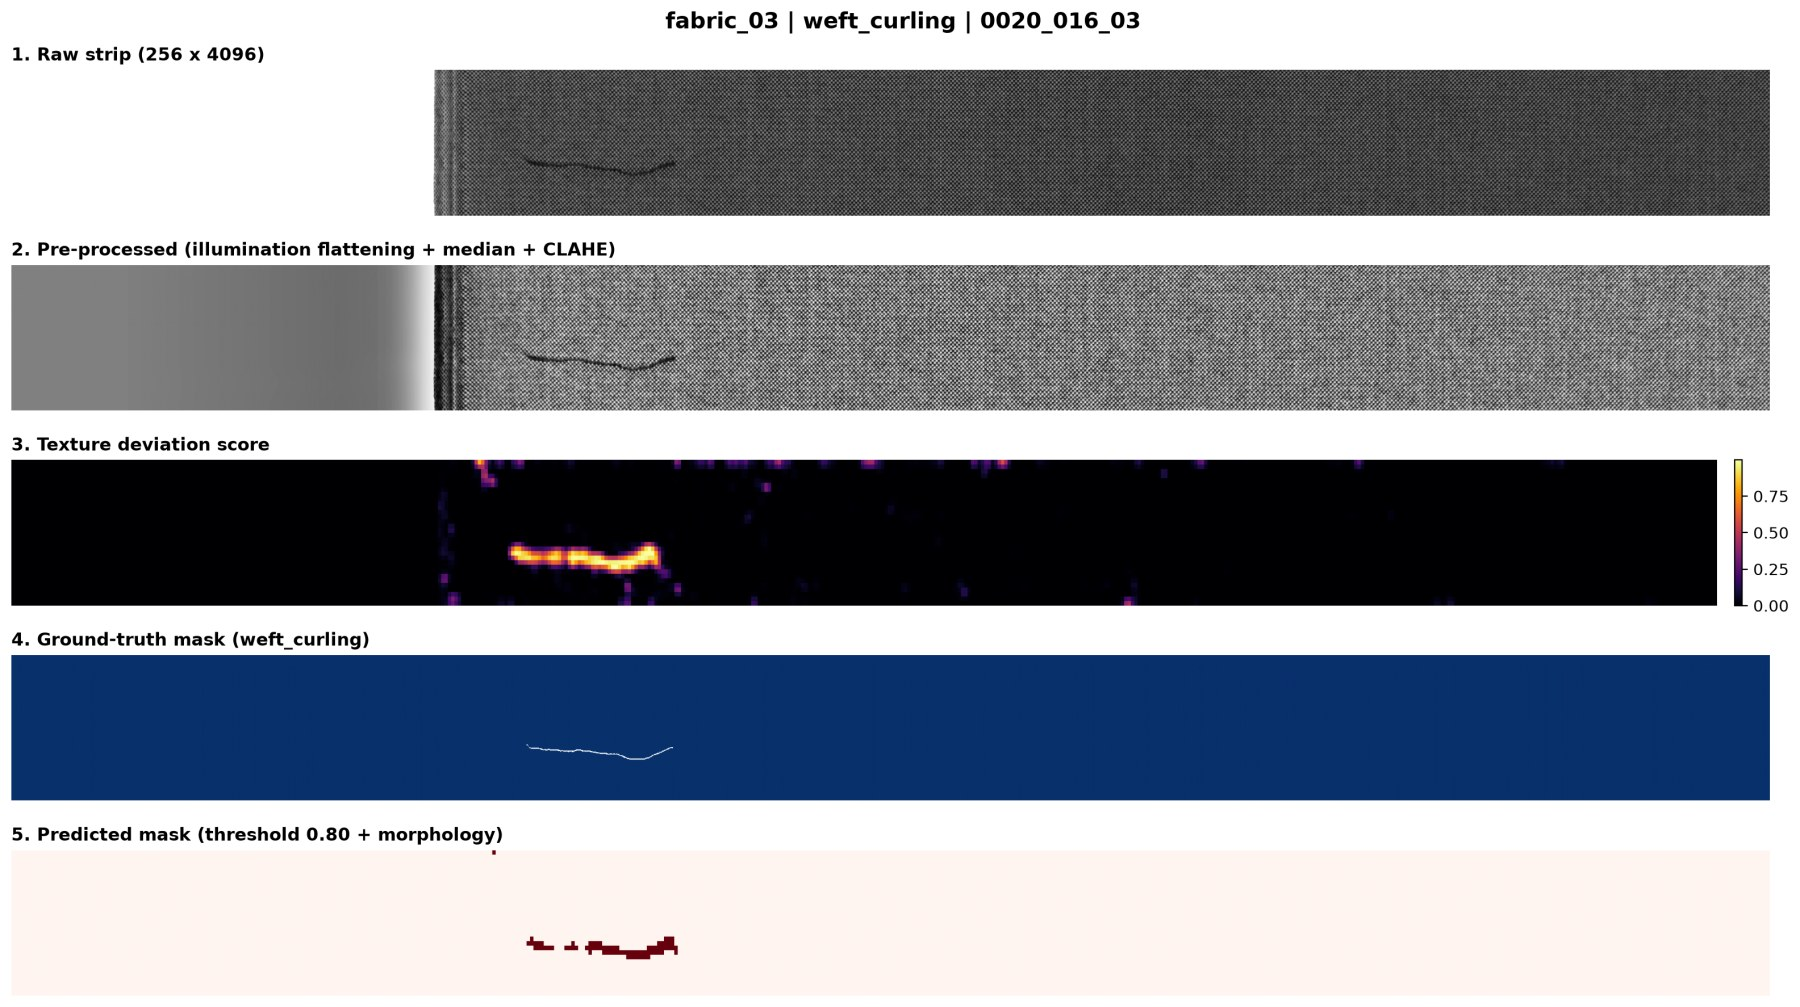
\includegraphics[width=0.95\textwidth]{figures/inspection_0020_016_03.jpg}
\caption{Weft curling, \code{0020_016_03} (fabric 03), scored by a model that never saw this strip. The $16\times16$ deviation map (panel~3) traces the curled weft along its whole length; the mask (panel~5) follows it with a few-pixel offset, which is exactly what the $\pm2$/$\pm3$\,px tolerance metrics forgive.}
\label{fig:curl}
\end{figure}

\begin{figure}[h]
\centering
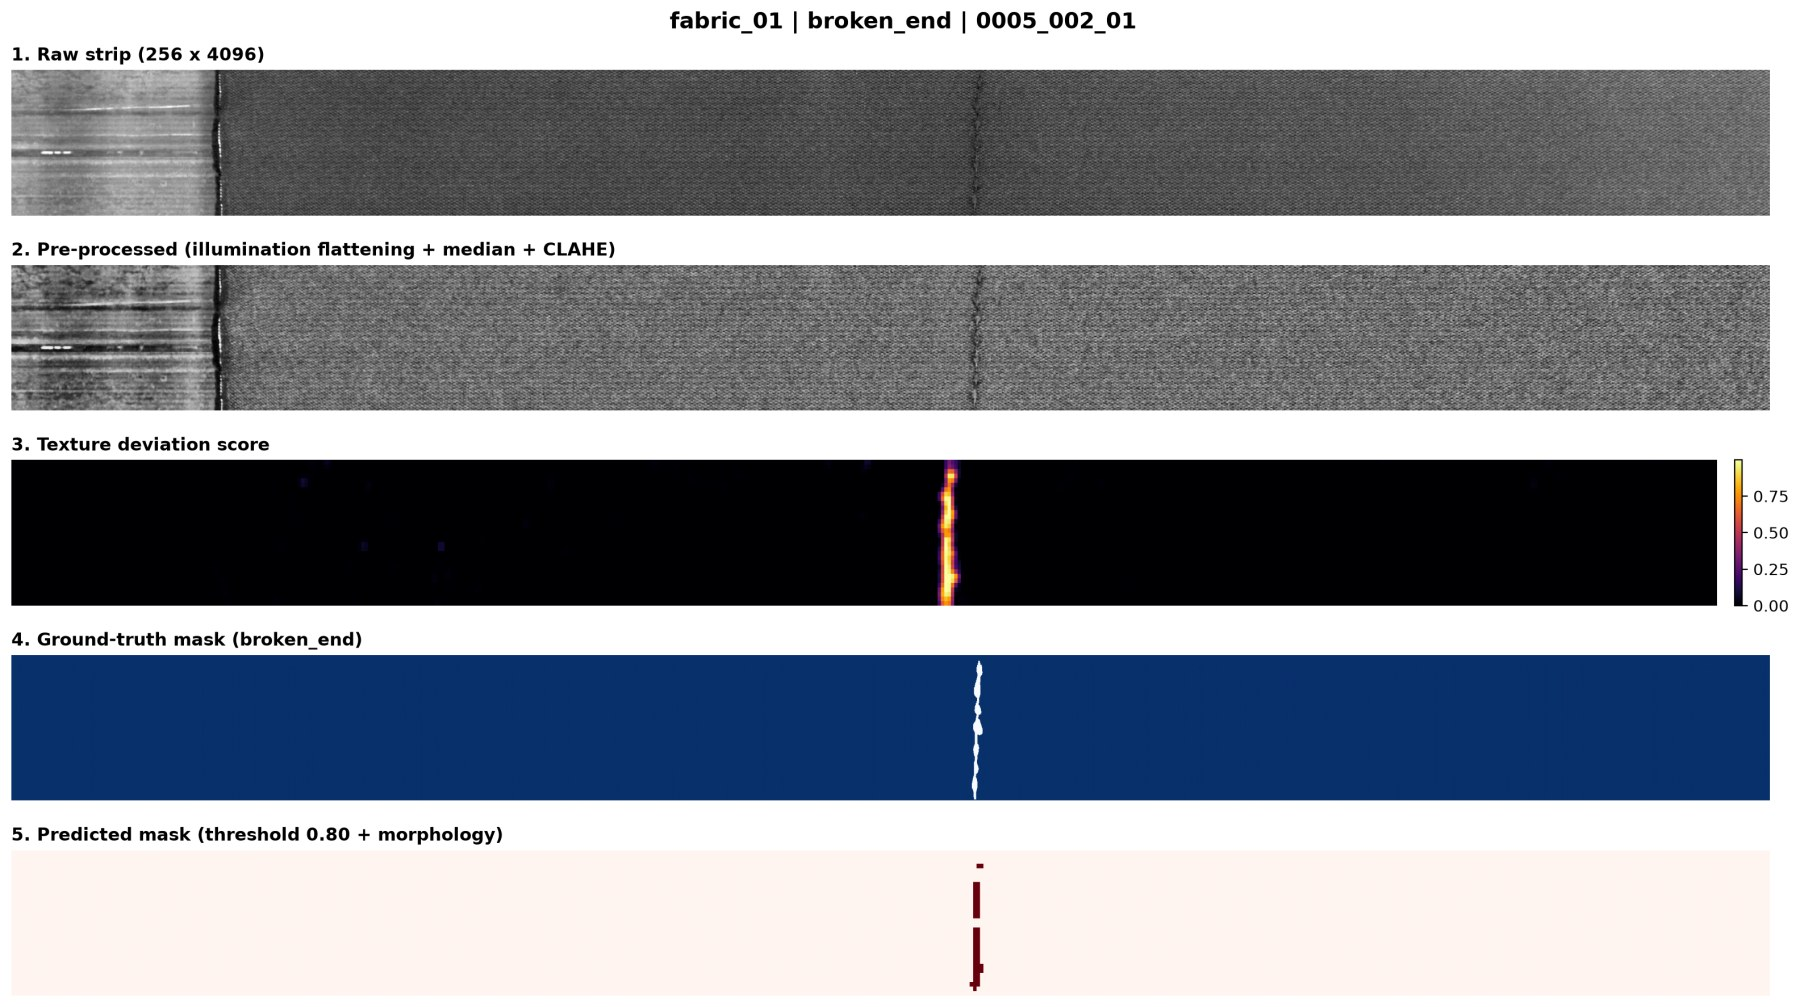
\includegraphics[width=0.95\textwidth]{figures/inspection_0005_002_01.jpg}
\caption{Broken end, \code{0005_002_01} (fabric 01). Compare with the Week~6 one-class result for broken ends, where the whole strip was flagged.}
\label{fig:end}
\end{figure}

\begin{figure}[h]
\centering
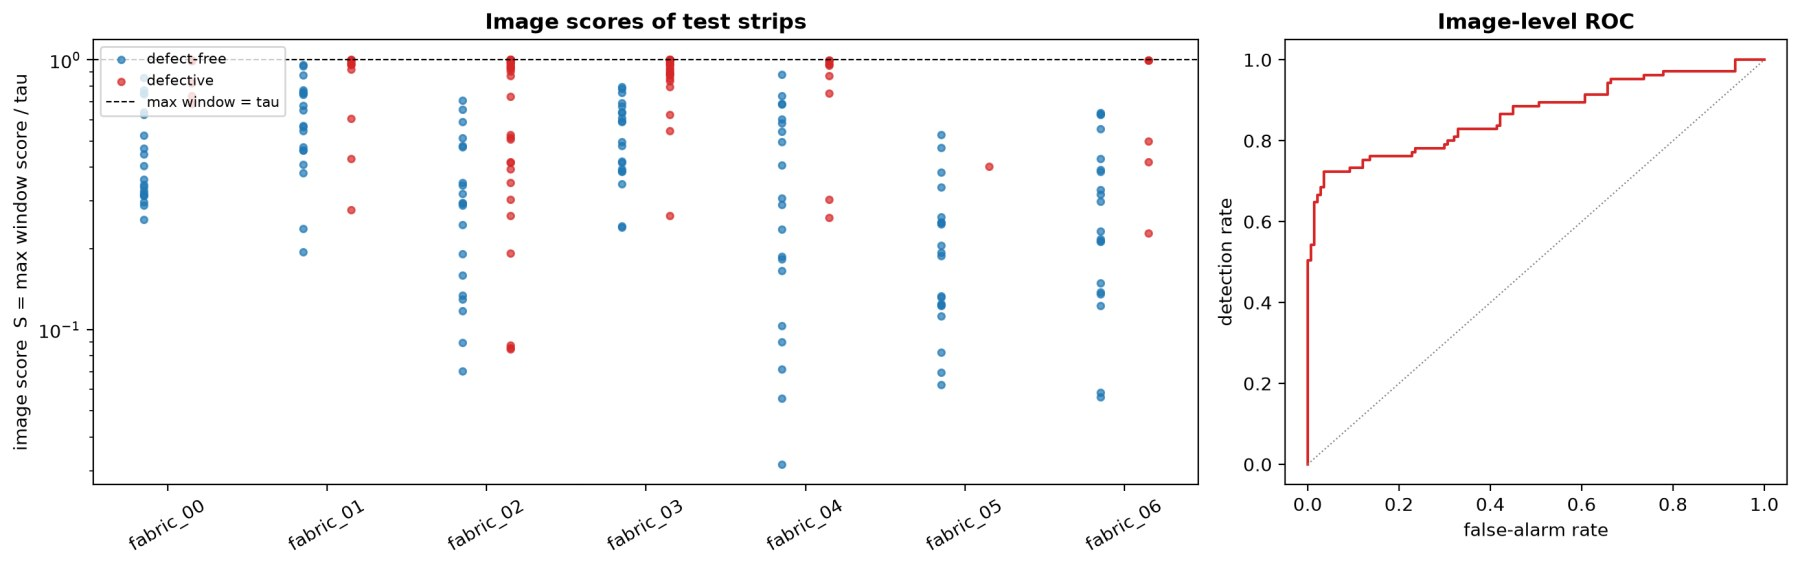
\includegraphics[width=\textwidth]{figures/image_scores.jpg}
\caption{Image scores (maximum window probability) of all 140 defect-free (blue) and 105 defective (red) strips per fabric, and the image-level ROC (AUROC 0.865).}
\label{fig:scores}
\end{figure}
\FloatBarrier
\section*{Discussion of Findings}
\begin{enumerate}
  \item \textbf{Learning what defects look like was the missing ingredient.} With the \emph{same} GLCM, LBP and Gabor descriptors, the window ranking rose from AUROC 0.536 (one-class, Week~7) to 0.980. The pooled pixel IoU rose about 19-fold (1.1 $\rightarrow$ 20.9\,\%), and the 256-patch F1 from 23.0 to 62.3\,\%. The descriptors were never the bottleneck. A model of normal texture alone could not separate defects from the AFID capture shift, while strip-normalised features plus labels can.
  \item \textbf{One strip dominates the pooled pixel numbers.} The weft crack \code{0080_036_01} has a 233{,}253-pixel mask, \emph{48\,\%} of all defect pixels in AFID's 105 masked strips. It is detected at image level, but only 0.6\,\% of its pixels are recovered; it alone explains fabric 01's 2.6\,\% pooled recall. Excluding that single strip, pooled pixel precision is 52.2\,\%, recall 49.1\,\%, F1 50.6\,\% and IoU 33.9\,\% (Table~\ref{tab:headline}). Both views are reported because neither alone is representative.
  \item \textbf{Thin defects are found but delineated a few pixels off.} Their pooled F1 rises from 34.5 to 40.4\,\% (precision 52.3 $\rightarrow$ 65.3\,\%) when a prediction within 3\,px of the true pixel counts as correct, the usual convention for thin structures.
  \item \textbf{Small blob defects remain hard.} Fuzzy balls (39 strips) reach only 6\,\% pooled IoU, although their window AUROC is 0.969. The detector finds \emph{where} they are, but 10--50\,px balls on a textured background cannot be outlined from $16\times16$ statistics, and the pixel filter bank rarely beat the window map on validation for them.
  \item \textbf{Validation chose different tools per fold.} The plain $16\times16$ map won in 3 of 5 folds, the pixel stage in 2, the 16/32 mean map once, and Hough linking in 3 (Table~\ref{tab:thr}). The added stages help on some data but are not uniformly better, which is why they are chosen on validation instead of being always on.
  \item \textbf{Image-level detection is real, not a capture artefact.} All 140 defect-free strips are now negatives, and the decision features are strip-normalised. Accuracy is 80.8\,\% overall and 88.2\,\% on fabric 03 (F1 90.3\,\%). Fabric 05 has a single defective strip, a knot that is never detected; that fabric is effectively untestable.
  \item \textbf{Limits of the evaluation.} With 105 defective strips over 12 classes, several classes have $n=1$ (knot, contamination, weft crack), so their per-class numbers are anecdotal. Cross-validation folds are stratified but small; the fold-to-fold spread of the chosen thresholds (Table~\ref{tab:thr}) shows that the operating point is not yet stable.
\end{enumerate}

\section*{Testing and Reproducibility}
The suite grew from 86 to 103 tests. New tests cover:
\begin{itemize}
  \item the filter bank: a full-width dark row lights up the weft channel and not the warp channel
  \item grid nearest-context lookup against a brute-force distance matrix
  \item per-strip window sampling (all positives kept, the negative floor respected, deterministic)
  \item the per-stratum fit/validation split, Hough linking (gaps filled, diagonals and out-of-region pixels untouched) and config validation
  \item an end-to-end supervised cross-validation through the CLI, checking that every strip is scored exactly once
\end{itemize}
Every result folder carries \code{run_config.json} (git SHA, full configuration) and \code{thresholds.csv}.

\section*{Commit History}
\begin{longtable}{@{}lp{0.80\textwidth}@{}}
\caption{Commits of the week on \code{feat/week-8} (one-line messages).}\label{tab:commits}\\
\toprule
\textbf{Hash} & \textbf{Message} \\
\midrule
\endfirsthead
\toprule
\textbf{Hash} & \textbf{Message} \\
\midrule
\endhead
\code{115c78c} & feat: add supervised window and pixel classifiers on classical filter-bank features \\
\code{86b2dc0} & feat: add strip-grouped cross-validated supervised pipeline with 16x16 windows and validated thresholds \\
\code{b19a4f4} & test: cover supervised sampling, context lookup, Hough linking and the CV pipeline \\
\code{991b952} & feat: report pixel precision, recall and F1 with 2 and 3 px tolerance \\
--- & results, Excel export, README, this report and the End-Semester report (see the pull request) \\
\bottomrule
\end{longtable}

\section*{Plan for the Final Week}
\begin{itemize}
  \item End-Semester report and presentation with the frozen protocol and these final tables.
  \item Merge the Week 8 pull request after team review.
\end{itemize}

\section*{Conclusion}
Week~8 replaced the one-class detector with a supervised classical detector built from the same texture descriptors, a per-pixel filter bank and Hough line linking. It was evaluated by strip-grouped cross-validation, with every threshold chosen on validation strips. Compared with the Week~7 one-class detector:
\begin{itemize}
  \item pixel IoU (pooled) rose from 1.1\,\% to 20.9\,\% (33.9\,\% without the one weft-crack strip that holds half of AFID's defect pixels), and pixel F1 reaches 40.4\,\% within 3\,px
  \item $256\times256$ patch F1 rose from 23.0\,\% to 62.3\,\%
  \item the window ranking now reaches AUROC 0.98
  \item image-level accuracy is 80.8\,\% over all 245 strips (88.2\,\% on fabric 03)
\end{itemize}
The detector now localizes most line defects accurately. Its remaining weaknesses are pixel recall on large low-contrast defects and the outlining of small blobs; both are stated as limitations in the End-Semester report.

\begin{thebibliography}{99}
\small
\bibitem{haralick1973} R.~M.~Haralick, K.~Shanmugam, and I.~Dinstein, ``Textural features for image classification,'' \emph{IEEE Trans.\ Syst., Man, Cybern.}, vol.~SMC-3, no.~6, pp.~610--621, 1973.
\bibitem{ojala2002} T.~Ojala, M.~Pietik\"ainen, and T.~M\"aenp\"a\"a, ``Multiresolution gray-scale and rotation invariant texture classification with local binary patterns,'' \emph{IEEE Trans.\ Pattern Anal.\ Mach.\ Intell.}, vol.~24, no.~7, pp.~971--987, 2002.
\bibitem{jain1991} A.~K.~Jain and F.~Farrokhnia, ``Unsupervised texture segmentation using Gabor filters,'' \emph{Pattern Recognit.}, vol.~24, no.~12, pp.~1167--1186, 1991.
\bibitem{friedman2001} J.~H.~Friedman, ``Greedy function approximation: A gradient boosting machine,'' \emph{Ann.\ Statist.}, vol.~29, no.~5, pp.~1189--1232, 2001.
\bibitem{ke2017} G.~Ke \emph{et al.}, ``LightGBM: A highly efficient gradient boosting decision tree,'' in \emph{Adv.\ Neural Inf.\ Process.\ Syst.~30}, 2017, pp.~3146--3154.
\bibitem{duda1972} R.~O.~Duda and P.~E.~Hart, ``Use of the Hough transformation to detect lines and curves in pictures,'' \emph{Commun.\ ACM}, vol.~15, no.~1, pp.~11--15, 1972.
\bibitem{matas2000} J.~Matas, C.~Galambos, and J.~Kittler, ``Robust detection of lines using the progressive probabilistic Hough transform,'' \emph{Comput.\ Vis.\ Image Underst.}, vol.~78, no.~1, pp.~119--137, 2000.
\bibitem{varma2006} S.~Varma and R.~Simon, ``Bias in error estimation when using cross-validation for model selection,'' \emph{BMC Bioinformatics}, vol.~7, art.~91, 2006.
\bibitem{silvestre2019} J.~Silvestre-Blanes, T.~Albero-Albero, I.~Miralles, R.~P\'erez-Llorens, and J.~Moreno, ``A public fabric database for defect detection methods and results,'' \emph{AUTEX Res.\ J.}, vol.~19, no.~4, pp.~363--374, 2019.
\end{thebibliography}

\end{document}
